\subsection{Principe de l'analyse lexicale}
Dans la conception d'un langage de programmation, l'analyse lexicale est une étape inévitable. L'objectif est de transformer une suite de mots, à savoir le code source, en une suite de \textit{tokens} qui seront plus facilement interprétables par une machine. Un \textit{token} un couple composé d'un nom et d'une valeur optionnelle. Par exemple, dans le langage C, les mots clé \textit{if}, \textit{while}, \textit{return}, les ponctuation, les noms de variable ou même les littéraux \textit{true}, \textit{8.23} ,\textit{"Hello World"} sont des tokens.

\begin{figure}[H]
    \centering
    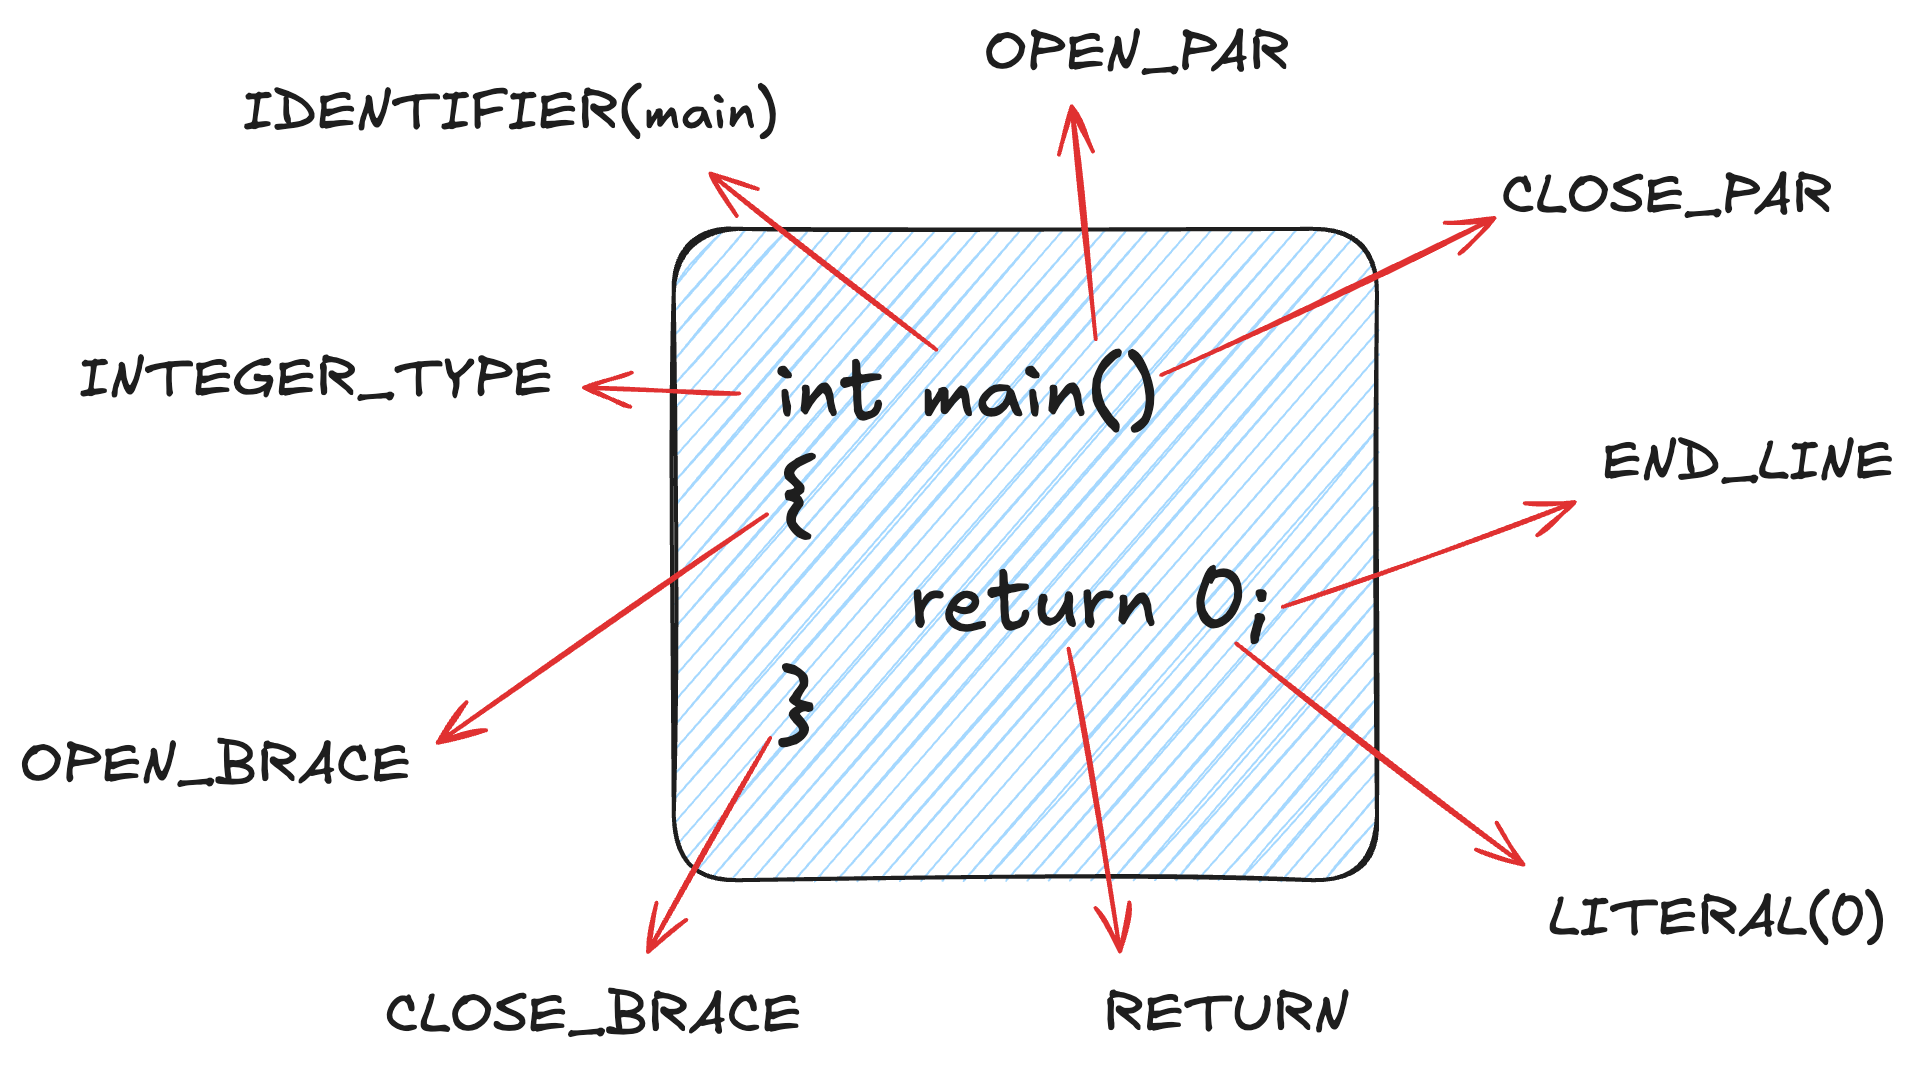
\includegraphics[width=12cm]{figures/syntaxe/lexing.png}
    \caption{Analyse lexicale d'un code en C}
    \label{fig2}
\end{figure}

C'est également à cette étape que certaines premières erreurs sont détectées, comme les erreurs de syntaxe. Par exemple, un mot clé ou un symbole non prévu par le langage va générer une erreur de syntaxe.

Certains tokens doivent cependant avoir une valeur associée pour être interprétables. Par exemple, un nombre entier doit être associé à une valeur numérique pour être utilisé dans un programme.

L'avantage des tokens par rapport au texte brut est que les tokens sont beaucoup plus facile à manipuler. Un exemple simple pour comprendre l'avantage des tokens est l'utilisation du signe \textquote{=} en C. Ce signe est utilisé pour l'affectation de variables, mais aussi pour la comparaison de deux valeurs. L'analyse lexicale permet de distinguer ces deux utilisations du signe \textquote{=}.

\subsection{Syntaxe d'Althread}
Dans le but d'obtenir un langage facile à prendre en main, la syntaxe d'Althread est proche de celle des langages existants comme le C, le rust et même promela dans certains cas. Cette section détaille les choix faits concernant la syntaxe du langage.

\subsubsection{Syntaxe pour les instructions}
Comme en langage C, les instructions en Althread sont séparées par un point-virgule.
\subsubsection{Structure du programme en blocks}
\subsubsection{Grammaire}

La grammaire d'un langage de programmation est la définition formelle du langage. Elle permet de définir les règles de syntaxe du langage et de déterminer si un programme est syntaxiquement correct.